\documentclass{beamer}
\usepackage{graphicx}
\usepackage{tcolorbox}
\usepackage{color,soul}
\graphicspath{ {./img/} }
\usetheme{Rochester}

\title{Pencarian File di Linux}
\author{Aldzikri Dwijayanto Prathama/195410189\\
		Rizqulloh Rifqi E/195410188\\
	M. Fadhillah F./195410197\\
Dimas Maulana A./195410198}

\begin{document}

\maketitle

\begin{frame}
    \frametitle{Pencarian Melalui Nautilus (GNOME 3.34)}
    \begin{columns}
        \column{.5\linewidth}
        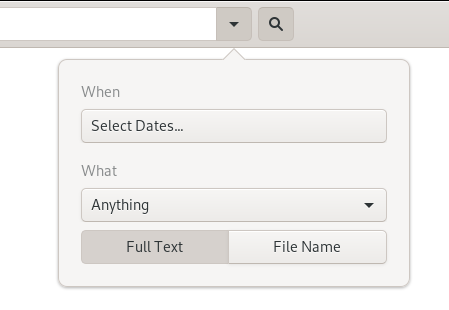
\includegraphics[width=\linewidth]{img1}
        
        \column{.5\linewidth}
        \begin{itemize}
        	\item Bisa langsung mengetik kata kunci yang inging dicari
        	\item Klik icon $\bigtriangledown$,  untuk opsi pencarian yang  lebih spesifik
        \end{itemize}
    \end{columns}
\end{frame}

\begin{frame}{Hasil Pencarian Nautilus}
	\begin{center}
		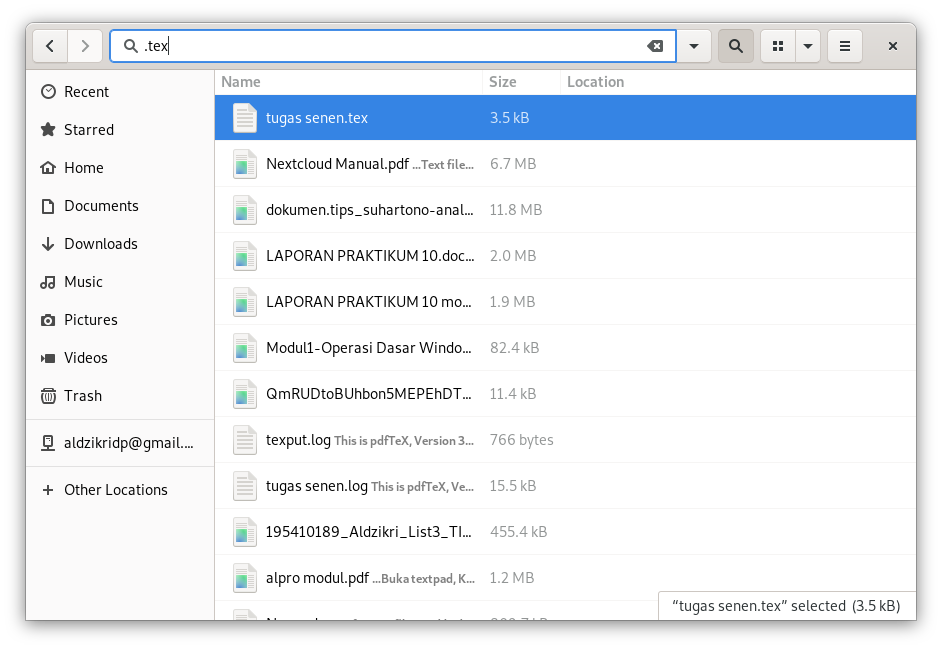
\includegraphics[scale=.3]{img3}
	\end{center}
\end{frame}

\begin{frame}
	\frametitle{Pencarian Menggunakan Perintah \texttt{find}}
	Struktur umum perintah \texttt{find}\\
	\begin{tcolorbox}
	\texttt{find options starting/path expression}
	\end{tcolorbox}
\begin{itemize}
	\item atribut \texttt{options} akan mengatur tindakan dan metode  yang dipakai oleh find
	\item atribut \texttt{starting/path} menentukan direktori find mulai mencari
	\item atribut \texttt{expression} mengatur apa yang akan dicari
\end{itemize}
	
\end{frame}

\begin{frame}{Opsi dan Optimisasi \texttt{find}}
	\begin{itemize}
		\item Secara default find mengabaikan symbolic link
		(file shortcut), untuk mencantumkan symbolic link tambah opsi \texttt{-L}
		
		\item Optimisasi \texttt{find} adalah strategi pencarian untuk meningkatkan kecepatan
		
		\item Tiga optimisasi yang dapat dipilih diantaranya \texttt{-O1}, \texttt{-O2}, dan \texttt{-O3}
	\end{itemize}
\end{frame}

\begin{frame}{Opsi dan Optimisasi \texttt{find}}
	\begin{itemize}
		\item \texttt{-O1} (Default) filter berdasarkan nama file terlebih dahulu                                  
		\item \texttt{-O2} File name terlebih dahulu, lalu type file                                               
		\item \texttt{-O3} Izinkan find untuk mengurutkan berdasarkan efisiensi sumber daya dan kemungkinan sukses
	\end{itemize}
\end{frame}

\begin{frame}{Contoh Perintah}
	\begin{tcolorbox}
		\texttt{find -O3 -L ~/Documents -name "*.tex"}
	\end{tcolorbox}
	Perintah ini mengaktifkan optiimisasi level maksimum (-O3), dan mengizinkan find untuk mengikuti symbolic links (-L). \texttt{find} akan mencari file yang berkahiran .tex di seluruh cabang direktori di bawah ~/Documents
\end{frame}

\begin{frame}{Contoh}
	Contoh hasil pencarian dengan find\\
	\begin{center}
		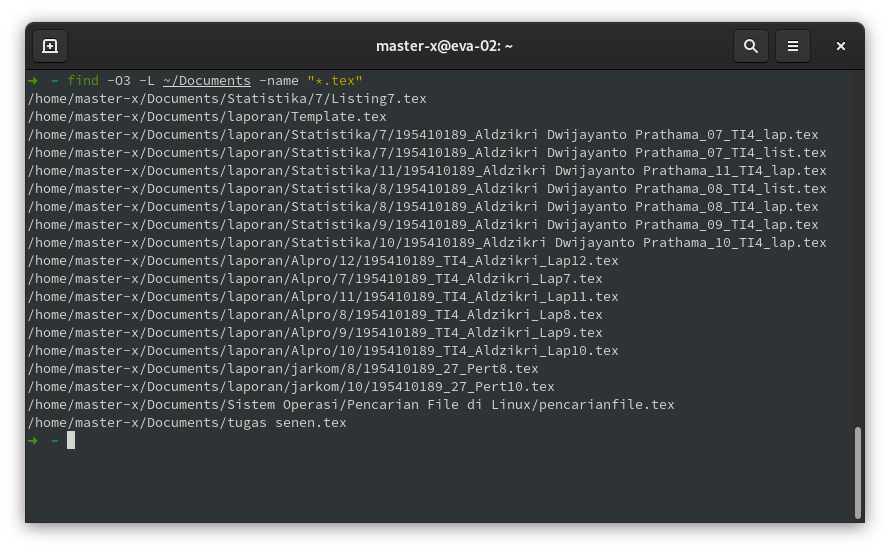
\includegraphics[scale=.3]{img2}
	\end{center}
\end{frame}

\begin{frame}{Manual \texttt{find}}
	Untuk opsi dan keterangan lebih lanjut, bisa membuka manual untuk find, dengan perintah
	\begin{tcolorbox}
		man find
	\end{tcolorbox}
	\begin{center}
		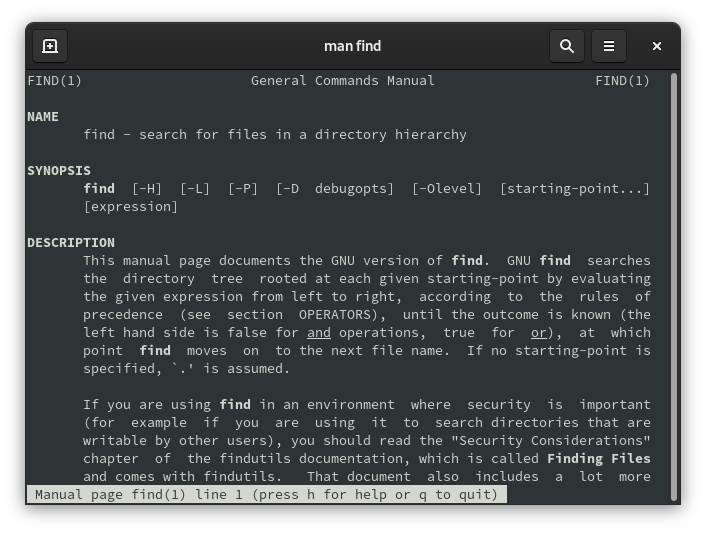
\includegraphics[scale=.25]{img4}
	\end{center}
\end{frame}

\begin{frame}{Referensi}
	\begin{itemize}
		\item find manual
		\item https://www.linode.com/docs/tools-reference/tools/find-files-in-linux-using-the-command-line/
	\end{itemize}
	
\end{frame}

\end{document}
